\documentclass{article}
\usepackage[utf8]{inputenc}
\usepackage{graphicx}
\usepackage{amssymb}
\usepackage{tabularx}
\title{Cognitive Science 1 \\ Final Study Guide}
\author{Benjamin Lee}
\date{March 2018}

\begin{document}

\maketitle

\section{Lectures 1-7}
Interdisciplinary approach to understanding \textbf{how} we think and \textbf{why} we perceive reality the way we do  \\

\begin{enumerate}
    \item Neuroscience: Explain cognitive processes mechanistically
    \item Psychology: Study cognitive processes behaviorally
    \item Computer Science: Build models of cognition and utilize biologically derived models to create "human" -like entities
    \item Linguistics: Use language generation and understanding to reveal how our minds interpret the world around us
    \item Philosophy: Build frameworks for understanding metaphysical components of cognition
    \item Social Science: Understand how cultural context affects cognition
\end{enumerate}

\subsection{CRUM Model}

\textbf{Central Hypothesis of Cognitive Science:} "Thinking can best be understood in terms of representational structures in the mind and computational procedures that operate on those structures" -Paul Thagard
\begin{itemize}
    \item When you think about something, you \textbf{represent} the ideas in some way and you operate on these ideas: 
    \item How to represent these ideas? \textbf{CRAPI}
    \begin{itemize}
        \item \textbf{Concepts:} formed through categorization; allows us to recognize members of category
            \subitem location: basal ganglia, prefrontal cortex
        \item \textbf{Rules:} Specify the relationships between propositions, if-then structures
            \subitem location: basal ganglia, prefrontal cortex
        \item \textbf{Analogies:} Target, source, comparison and mapping, and solution
            \subitem location: left prefrontal cortex
        \item \textbf{Proposition:} can specify all of the possible relationships between concepts (can be true or false)
            \subitem location: left hemisphere
        \item \textbf{Images:} complement verbal representation, but doesn't replace them; inspect, find, zoom, rotate, transform
            \subitem location: occipital lobe
    \end{itemize}
\end{itemize}

\noindent Ex: Think about a dog walking across the street. \\

I can represent a dog as a concept. The concept of dog has several properties such as: breed, name, color, x-pos, y-pos. \\

To think about the dog walking across the street, I will operate on my instantiation of the dog concepts by accessing the x-pos, y-pos properties and add or subtract value to it to move the dog in space. \\ 

\noindent Practice Ex: How might a student choose what class to take? \\ 

First, the student can represent classes as concepts, with properties such as subject, class size, time slot, etc. Then we can use propositions to compare our concepts to generate a sort of rank for schedule of classes. To pick the classes, we could use rules and proposition to compare the types of classes and compute a process of elimination. Analogies may also help identify which classes are like others and readjust ranks of classes as well as eliminate. 

\subsection{Localization of Function}
\begin{itemize}
    \item \textbf{Phrenology:} Idea by Franz Joseph Gall where the shape and size of the head determines the mental ability of a person. This idea was debunked, however, it lead to the idea of localization of functions in the brain. 
    \item \textbf{Karl Lashley:} searched for the engram of memory in the brain. Did an experiment with rats and mazes, lesioned the rats brain and tested it's memory of the maze, but it was still able to traverse the maze. Lead to the idea of distributed memory across the neocortex.
    \item \textbf{Wilder Penfield:} Electrically stimulated brain to discover which parts of the brain correlated to the parts of the brain. Was able to map the brain to functions of the body (creation of cortical homunculus) 
\end{itemize}

\noindent\textbf{Case Study: Phineas Gage}
\begin{itemize}
    \item Helped represent this idea of localization of function
    \item Used to be a great leader and supervisor of his men on railroad
    \item Accident lead to his entire right frontal lobe to be destroyed. 
    \item Gage could no longer function, loss of planning, social skills, highly irritable. 
\end{itemize}

\subsection{Regions of the Human Brain}
\textbf{4 major regions of the brain}
\begin{itemize}
    \item Frontal Lobe: motor function, problem solving, spontaneity, memory, language, initiation, judgment, impulse control, and social and sexual behavior.
    \item Parietal Lobe: Motor cortex (anterior) and somatosensory cortex (posterior) 
    \item Temporal Lobe: sensory information from ears, language, consolidation of memory
    \item Occipital Lobe: visual processing
\end{itemize}

\subsection{Structure and function of neurons (action potentials)}

\begin{figure}[htp]
\centering
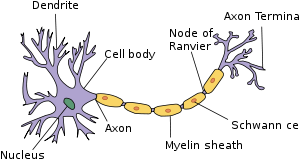
\includegraphics[width=8cm]{images/neurons.png}
\caption{Neuron}
\label{fig:neuron}
\end{figure}

\textbf{Action potentials} are formed when the summation of EPSPs and IPSPs passes the threshold. Carries information within the neurons via electrical impulses \\

\textbf{Myelin} are fatty sheaths that insulate some neurons. Insulation increases the speed of conductance of electrical impulses (saltatory conduction) 

\subsection{Eric Kandal and Hebbian Learning}
\textbf{Hebb's Rule:} "neurons that fire together wire together" 

\begin{itemize}
    \item \textbf{Hebbian Learning:} strengthening synaptic connections
    \item Eric Kandal and Aplysia Californica slugs: provided evidence for the involvement of Hebbian learning mechanisms at synapeses. 
        \subitem Shocked the gills of the slug which reacted by closing its gills. When doing this multiple times it strengthened its retraction. 
\end{itemize}

\subsection{Brain Mapping Techniques}

Structural imaging: used to image the brain and locate lesions, tumor etc \\
\noindent Functional Imaging: used to detect functions of brain processes and measure brain activity \\

\noindent Concerned with three things when measuring brain activity 
\begin{itemize}
    \item \textbf{Temporal Resolution:} refers to the accuracy with which one can measure "when" an event occurs
    \item \textbf{Spatial Resolution:} refers to the accuracy with which one can measure "where" an event is occurring
    \item \textbf{Invasive:} refers to whether or not equipment is located "internally or externally" 
\end{itemize}

\noindent\textbf{Brain Imaging Tech:}
\begin{itemize}
    \item Electroencephalogram (EEG): measures the gross electrical activity of the entire brain; more temporal, less spatial
    \item Computer Axial Tomography(CAT): uses x-rays and images the brain on axis (triangulation). structural, faster than MRI but less info b/c combination of x-ray images from 3 different axis
    \item Positron Emission Tomography (PET): injects radioactive isotope for a specific neurotransmitter and uses radioactive detectors to locate receptors of neurotransmitter. functional and BOLD measurement
    \item Magnetic Resonance Imaging (MRI): soft tissue structure is measurd by the alignment of protons using a powerful magnet (structural) 
    \item functional MRI (fMRI): shows changes in brain activity "over time" using same technique but for hydrogen b/c water in blood. functional; high spatial, low temporal 
    \item Transcranial Magnetic Stimulation: non-invasive method to excite neurons in the brain: weak electric currents are induced in the tissue by rapidly changing magnetic fields
\end{itemize}

\noindent\textbf{More Brain imaging techniques and spatial resolutions}\\
\begin{tabularx}{\textwidth}{|c|c|c|c|c|}
    \hline
    Method & Application & Spatial Resolution & Temporal Resolution & Invasiveness  \\
    \hline
    EEG & Functional & poor (cm's) & moderate (100's ms) & non-invasive \\
    ECoG & Functional & moderate (100's $\mu$m to mm's) & good (ms's - 10's ms) & over cortex\\
    MRI & Structural & moderate & N/A & non-invasive \\
    fMRI & Functional & moderate & poor (seconds) & non-invasive \\
    MEG & Functional & moderate & good & non-invasive \\
    PET & Functional & moderate & poor & injects rad isotope \\
    CT (CAT) & Structural & moderate & N/A & uses x-rays\\
    Patch clamp & Functional & Excellent ($\mu$m to 100's $\mu$m) & Excellent (ms) & Penetrates neuron\\
    \hline
\end{tabularx}
\bigskip

\noindent\textbf{Types of Glial Cells:}
\begin{itemize}
    \item \textbf{Oligodendrocytes:} provide insulation (myelin) to neurons (brain) 
    \item \textbf{Astrocyte:} star shaped cells that provide physical and nutritional support for neurons
    \item \textbf{Microglia:} Like astrocytes, also digest parts of dead neurons (janitorial service) 
\end{itemize}

\nondent \textbf{Albert Einstein's brain:} had more connections in corpus callosum and more glial cells in brain 

\subsection{Split Brain Research}
Roger Sperry's experiments
\begin{itemize}
    \item Patients corpus callosums were split because they had severe seizures which transferred across the brain and severing the connection between the hemispheres significantly reduced them. 
    \item Experiment involved flashing two words in each field of vision and asking patients to say what they saw. 
    \item He was able to say ring, because speech is located in the \textbf{left hemisphere} and the word ring was in his \textbf{right field of vision}
    \item However he could not say key which showed up in his \textbf{left visual field}, because there is no communication across the hemispheres, but he could identify the object with his \textbf{right hand}
\end{itemize}
 Left brain functions: analytic thought, logic, language, science and math\\
 Right brain functions: holistic thought, intuition, creativity, music

\subsection{Neural Interfaces}
\textbf{Neural Interface:} a system which can communicate with the nervous system \\

\noindent Useful for projects such as the \textbf{CoLBeRt System:} Controlling Locomotion and Behavior in Real Time \\
Scientists are using CoLBeRT to understand how a handful of neurons can work together in an animal to generate behavior \\

\noindent\textbf{Four Factors when choosing Neural Interface:}
\begin{itemize}
    \item \textbf{Spatial/Temporal Resolution:} minimum physical space and time in which a signal can be distinguished
    \item \textbf{Device/System Lifetime:} How long can your interface interact with nervous system before it degrades?
    \item \textbf{Invasiveness:} How much damage or potential damage to the body occurs with implementation of your interface?
    \item \textbf{Functionality:} 
    \begin{itemize}
        \item \textbf{Record:} can you detect neuronal activity?
        \item \textbf{Stimulate:} Can you trigger neuronal activity?
        \item \textbf{Block:} can you prevent neuronal activity?
    \end{itemize}
\end{itemize}

We care about the spatiotemporal resolution of a neural interface to get clear signals that we can interpret with our interfaces. The more distorted our information is, the harder it is for our interfaces to perform functions \\

We have tools with different spatiotemporal resolutions because they have various levels of invasiveness, functionality, and lifetimes. For example, magnetic resonance is non-invasive, but has poor spatiotemporal resolution. Ephys is very invasive, begin directly snapped onto a neuron or in the brain but produces high spatiotemporal resolution, but the lifetime is poor as it can degrade. \\

Neural interfaces fail because the only good ones are the invasive ones and that is not preferred by subjects. There also aren't very good Neural interfaces out there that produce the best preferences. \\

Ethical concerns with BMI systems include who gets access to a persons brain waves, deep personal thoughts and dreams that shouldn't be viewed by other people, etc. Access to brain waves and our most private thoughts is more dangerous in the hands of companies than say our Facebook posts. 

\subsection{David Marr's model of vision}

\begin{figure}[htp]
\centering
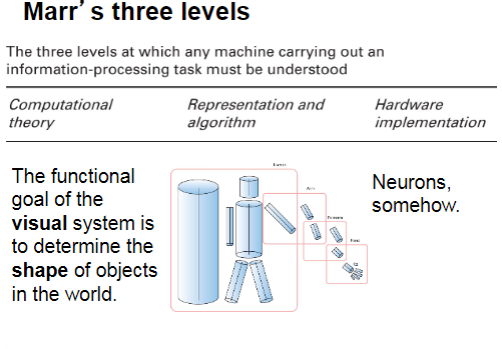
\includegraphics[width=\textwidth]{images/marrsvision.PNG}
\caption{Marrs 3 levels of vision}
\label{fig:neuron}
\end{figure}

\subsection{Visual Pathway}
Retina $\rightarrow$ LGN $\rightarrow$ Primary visual cortex (V1) 

\begin{itemize}
    \item \textbf{Retina:} consists of a layer of photoreceptors at the back of the eyeball
    \item \textbf{Lateral Geniculate Nucleus (LGN):} Located in the thalamus, which is a sort of relay station for the brain (5 senses, except smell) 
    \begin{itemize}
        \item P-type ganglion cells (\textbf{Parvocellular}): Shape, layers 3-6
        \item M-type ganglion cells (\textbf{Magnocellular}): Motion, layers 1-2 
        \item NonM-NonP ganglion cells (\textbf{Koniocellular}): Color, all layers
    \end{itemize}
    \item \textbf{Primary visual cortex (V1):} also known as striate cortex. Contains \textbf{simple cells} and \textbf{complex cells} for detecting orientation and directional sensitivity, in order. 
    \item \textbf{Extrastriate cortex:} V2, V3, V4, V5
    \begin{itemize}
        \item V2: cells are tuned to simple properties such as orietation, spatial frequency, and color
        \item V3: decides whether dorsal (where) vs. ventral(what) 
        \item V4: "What" helps determine what you are seeing
        \item V5: "where" perception of motion, the integration of local motion signals into global percepts and guidance of some eye movements
    \end{itemize}
\end{itemize}

\noindent\textbf{Dorsal Stream ("where"):} Associated with motion, representation of objects locations, and control of the eyes and arms \\
\textbf{Disorders:}
\begin{itemize}
    \item \textbf{Akinetopsia:} motion blindness, disjointed movement
    \item O\textbf{ptic Ataxia:} deficit in visual guided reaching (grabing water bottle, walking) 
\end{itemize}

\noindent\textbf{Ventral Pathway ("what"):} associated with form recognition and object representation, also with storage of long term memory. \textbf{Fusiform gyrus} activates when recognizing these objects or faces.\\
\textbf{Disorders:}
\begin{itemize}
    \item \textbf{Achromotopsia:} color blindness: inability to perceive color
    \item \textbf{Prosopagnosia:} faceblindness: can see face, but cannot recognize (hard to perceive faces upside down as well) 
\end{itemize}

\noindent 90\% of the information from our retina goes to the striate cortex (V1), the conscious visualization \\
The other 10\% goes to the \textbf{superior colliculus} which is the unconscious part. Animalistic instinct sort of reaction, noticing movement and such not in our field of consciousness. 

\subsection{Memory}
\begin{itemize}
    \item \textbf{Retrograde Amnesia:} Loss of memory events prior to the occurrence of the brain damage
    \item \textbf{Anterograde Amnesia:} the loss of the ability to form new memory after brain damage occurred
\end{itemize}

\noindent\textbf{Case Studies:}
\begin{itemize}
    \item \textbf{Kim Peek (savant):} savant is a condition which a person with mental disability demonstrates profound ad prodigious capabilities or abilities. In his case, his corpus callosum never formed, instead his two hemispheres fused together (90\% connection) which allowed him to remember things fairly well, although could not function "normally"
    \item \textbf{Clive Wearing:} suffers from both anterograde and retrograde amnesia 
    \begin{itemize}
        \item insight into how memory is distributed and not localized in hippocampus. 
        \item procedural memory is still intact, plays piano, remembers wife. 
    \end{itemize}
    \item \textbf{H.M.:} Had his hippocampus and medial temporal lobe removed
    \begin{itemize}
        \item had massive anterograde amensia (couldn't form new memories) 
        \item episodic and semantic memory difficult, but procedural fine (could remember tasks using procedural, but not much else) 
        \item led to idea of hippocampus being need for consolidation of information from STM to LTM
    \end{itemize}
\end{itemize}

\textbf{Tulving Model}
\begin{figure}[htp]
\centering
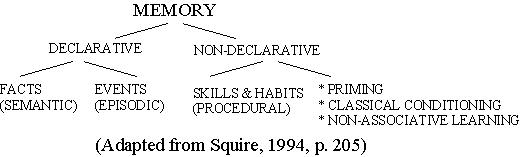
\includegraphics[width=\textwidth]{images/tulving_model.jpg}
\caption{Tulving Model}
\label{fig:tulving}
\end{figure}

\bigskip

\textbf{The Modal Model} \\
\begin{figure}[htp]
\centering
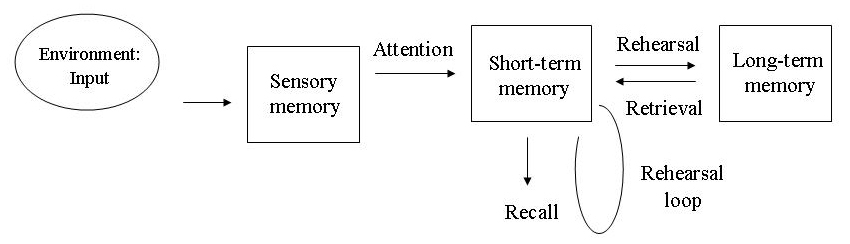
\includegraphics[width=\textwidth]{images/modalmodel.jpg}
\caption{The Modal Model by Atkinson and Shiffrin 1968}
\label{fig:modal}
\end{figure}

\textbf{Short term memory:} 
\begin{itemize}
    \item Limited duration(seconds), improved with rehearsal/repetition
    \item limited capacity, use chunking to meaningfully group
    \item coding can be acoutic visual or semantic
\end{itemize}
\textbf{Iconic Memory:} Brief persistence of visual impression \\
\textbf{Echoic Memory:} transient auditory memory

\subsection{Sleep}
\noindent\textbf{Stages:}
\begin{itemize}
    \item \textbf{Non-Rapid Eye movment sleep (NREM):} stages 1-4, deeper sleep the higher the number. Stages 3-4 are "Slow Wave Sleep" (SWS)
    \item \textbf{Rapid Eye movement sleep (REM)}
    \item Start at REM and slowly go down to NREM stages
    \item NREM to REM sleep cycle is 90 minutes in humans
\end{itemize}

\noindent\textbf{Sleep and Memory:} Sleep helps stabilize and consolidate memory
\begin{itemize}
    \item \textbf{NREM SWS} is most helpful in retaining and consolidating memory
    \item enhancing SWS increases consolidation of declarative memories
    \item Pulling all-nighters significantly effects your memory as the consolidation part is not there. Memory must be transferred to long term during sleep. 
    \item Motor skill learning correlates to stage 2 NREM late in the night
    \item Visual skill consolidation correlates with the combination of early SWS and late REM (between REM and stage 2-3ish)
\end{itemize}
\noindent\textbf{REM Sleep:}
\begin{itemize}
    \item Areas activated by REM sleep: 
    \begin{itemize}
        \item  emotional regulation (cingulate cortex)
        \item movement initiation (motor cortex) 
        \item Complex visual processing (occipital cortex) 
        \item Emotion (aymgdala)
        \item Memory (hippocampus) 
    \end{itemize}
    \item Areas deactivated by REM: logical reasoning (lateral prefrontal cortex) 
   \item REM sleep: the perfect emotional balm, time heals wounds
\end{itemize}

\section{Lecture 8: Categories and Stereotypes}
What are \textbf{concepts}? 
\begin{itemize}
    \item Concepts are thoughts and can be used to \textbf{build relationships} between thoughts
    \item Concepts are the elements of reason and constitute the \textbf{meaning of words and linguistic expressions}
    \item In short: Mental representations that enable individuals to categorize objects in one way or another.
\end{itemize}
\textbf{Categorization:} the capacity to systematically group events and objects \\

\subsection{3 Approaches to Categorization: Exemplar, Feature, Prototype}

\noindent \textbf{Exemplar (experiences):}
\begin{itemize}
    \item Categorization involves comparing some object or event with previous instances stored in memory 
    \item Example: I categorize some new animal as a dog if it matches with previous instances of dogs I've stored in memory
    \item Similarity to instances already formed: 
        \subitem Based on experience
        \subitem Con: Categories $\rightarrow$ realize something belongs to a category but haven't seen it before
    \item Difficulty: within a category, the entities are very different from each other
\end{itemize}

\noindent \textbf{Feature (Classical View):}
\begin{itemize}
    \item Categorization of objects and events is based on a set of \textbf{necessary and sufficient conditions} for category membership
    \item Example: the category bachelor must be adult, human, male, unmarried, in order to qualify for membership. 
    \item All features must be present (equal membership)
    \item Clear-cut (no fuzzy boundary)
\end{itemize}

\noindent \textbf{Prototype:}
\begin{itemize}
    \item Categorization takes place on the basis of a prototype, a highly salient or typical member of the category (average member)
    \item Example: I categorize an object as a chair depending on the degree to which it looks like a typical chair. Typical dog, house, summer day, etc. 
    \item Some members of a category are more typical than others 
    \item Fuzzy boundary (not clear or exact)
\end{itemize}

\subsection{Graded Membership and Family Resemblance}

\begin{figure}[htp]
\centering
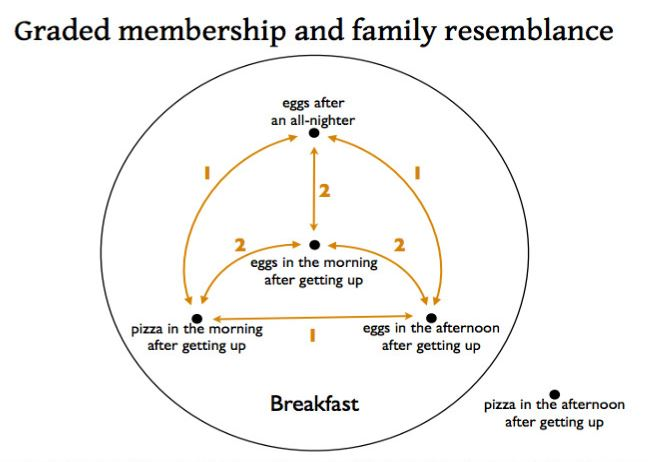
\includegraphics[width=10cm]{images/Breakfast.JPG}
\caption{Graded membership}
\label{fig: Graded Membership}
\end{figure}

\noindent \textbf{Graded membership:} Some members are better than others, (certain categories are held in a higher regard than others) \\
\textbf{Family resemblance:} things in the category share features with each other. (Example: eggs are related to breakfast, which is what you eat in the morning, after waking up) \\
\textbf{Fuzzy boundaries:} hard to identify the boundary (Example: you can have pizza in the morning and still consider it breakfast.) \\

Prototypical breakfast: 
\begin{itemize}
    \item Eaten early in the day
    \item after a period of sleep 
    \item has a special menu (eggs, toast, etc)
    \item remove any feature and we still have a breakfast of some sort (can't remove 2 or more features or else it won't be breakfast anymore)
\end{itemize}
\textbf{Heuristic search} (not perfectly accurate search but close enough and fast) \\

\noindent Misleading of prototypes: 
\begin{itemize}
    \item Conjunction fallacy
        \subitem It is impossible for the conjuction of two conditions to be more probable than either conjunction alone, but people still fall under the pretense that a category has both these conditions 
\end{itemize}

\begin{figure}[htp]
\centering
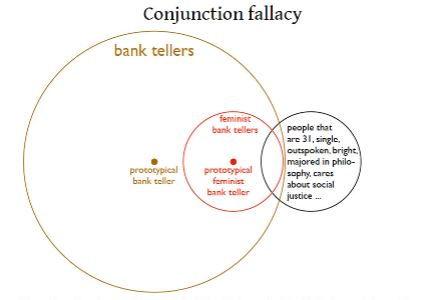
\includegraphics[width=10cm]{images/conjunctionfallacy.JPG}
\caption{Conjunction Fallacy Example}
\label{fig: conjunction}
\end{figure}

\subsection{Hierarchy in Categorization: Superordinate, Basic-level, Subordinate}

\begin{figure}[htp]
\centering
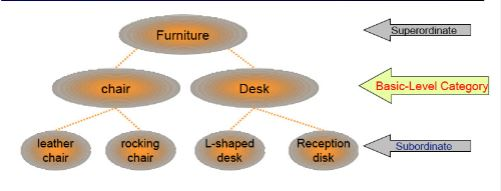
\includegraphics[width=10cm, height=5cm]{images/prototypelevel.JPG}
\caption{Categories and Prototypes: levels}
\label{fig: categories}
\end{figure}

\begin{itemize}
    \item \textbf{Superordinate} (superordinate semantic category)
        \subitem Category at the top from which the others branch out
        \subitem Most general level of a categorization (i.e. Furniture)
    \item \textbf{Basic-Level}
        \subitem more specific category to superordinate (ex. chair or desk) 
    \item \textbf{Subordinate} (semantic category) 
        \subitem specific level usually "type of" (ex leather chair, rocking chair) \\
        
\textbf{Three ways of examining the categories we form: }
    \subitem relations between categories (basic-level category) 
    \subitem internal category structure (radial category) 
    \subitem instances of category members (prototypes) 
\end{itemize}

Categorization has been noted to have some sort of hard-wiring before we are even born. By age 3 or even infancy, children classify the people they meet into groups. \\


\newpage 
\section{Lecture 9: Linguistics: Aphasias, Metaphors}

\textbf{Language is special:}
\begin{enumerate}
    \item Relies on \textbf{mental representations} (trouble for behaviorism) 
    \item Particular strengths and weaknesses: great for things that aren't here
    \item Uniquely \textbf{human}: suggests an innate basis, trouble for empiricism (all knowledge is derived from sense-experiences (John Locke, George Berkeley, David Hume) )
    \item \textbf{Potentially infinite}: can always produce novel sentences
\end{enumerate}

\subsection{B.F. Skinner's Radical Behaviorism}
\begin{itemize}
    \item Worked on classical conditioning 
    \item Dispenses with talk of mental states
    \item Aims to explain behaviour in terms of the environment
    \item "recognizes \textbf{no dividing line} between man and brute"
\end{itemize}
 
stimulus $\rightarrow$ \framebox{organisms mental state} $\rightarrow$ response

\subsection{Broca's Area \& Wenicke's Area; corresponding aphasias}
 
\textbf{Aphasia:} "without/lacking speech" \\
 
\noindent \textbf{Broca's Area:}
\begin{itemize}
    \item Involved in speech production (ability to produce spoken language) 
    \item Located in left frontal hemisphere
    \item \textbf{Broca's Aphasia:} damage to Broca's area results in the loss of speech production
\end{itemize}
 
\noindent \textbf{Wernicke's Area:}
\begin{itemize}
    \item Involved in the comprehension/understanding of spoken language
    \item located in left temporal lobe 
    \item \textbf{Wernike's Aphasia:} damage to Wernicke's area results in loss of language comprehension. May sound fluent in language, but lacks all meaning. 
\end{itemize}

\noindent \textbf{Kim et al.(1997):} Used fMRI to investigate multiple languages in brain 
\begin{itemize}
    \item Anatomical separation of the two languages in Broca's area varies depending on the time the second language was acquired. (early childhood or adulthood)
    \item Age may be signnificant inn lannguage functional organization. 
\end{itemize}

\noindent \textbf{Alexia:} the individual cannot read but can still write \\
\textbf{Agraphia:} the individual can reason normally, but cannot write \\
 
\noindent \textbf{Chomsky's Universal Grammar:} proposes a set of rules intended to explain language acquisition in child development \\

\noindent \textbf{Recursion:} 
\begin{itemize}
    \item Sentences are formed from clauses 
    \item The property of a system that permits the embedding of an element of the system within itself 
    \item Essentially, you can continuously create endless sentences with no semantics
    \item Example:
        \subitem This is the house that Jack built.
        \subitem This is the cheese that lay in the house that Jack built.
\end{itemize}

\noindent \textbf{Critical Period:} If linguistic experience is missing in the critical period (early childhood) language ability is impaired. \\
Case Studies: Victor the "wild child" and Genie \\

\noindent \textbf{Mirror Neurons:} Neurons fire when you see action or perform it
\begin{itemize}
    \item Found on accident when researchers were eating a banana in front of a monkey. They left the probe in the monkey and it started firing while the monkey watched them eat a banana. 
    \item Firing thought to be implicated in imitation (crucial ability for learning) 
    \item When areas inn which mirror neurons are located are anatomically connected, they form a mirror neuron system (MNS)
\end{itemize}

\textbf{George Lakoff's Brain Conncept Article:} proposes that the sensory-motor system has the right kind of structure to characterize both sensory-motor and more abstract concepts. \\

\textbf{Key Figures:}
\begin{itemize}
    \item \textbf{Noam Chomsky}
        \subitem View: Humans have innate "language faculty" and that the universal principles of human language reflect intrinsic properties of this language faculty
        \subitem Language is autonomous and separate from concepts
        \subitem Since we can create sentences that have no meaning recursively and endlessly, we can separate syntax and semantics
    \item \textbf{George Lakoff}
        \subitem Aims to link language to everyday thinking. Language recruits perceptual and cognitive processes, and is grounded in our everyday embodied experience. 
        \subitem Meaning is conceptualization (ex: same image can have multiple meanings)
        \subitem Since language derives from meaning, (as in language has to have some meaning because without meaning why would there be language) then we cannot separate syntax and semantics. 
\end{itemize}

\newpage
\section{Lecture 10: Cognitive Linguistics with Teenie Matlock}

\textbf{General goal of Cognitive Linguistics:} Sought deeper explanations and wanted to link language to everyday thinking, link between language and cognition \\
\indent -Focus on semantics mostly\\
\indent -Meaning is dynamic, deep, and bound in our experience \\

\textbf{Spatial metaphors:} those metaphors that have space as their source domain and map the image-schematic structure of space onto that of nonspatial and typically abstract target domains, thus enabling the user to talk about and perhaps even to think of those nonspatial domains in spatial terms. \\

\subsection{Metaphors of motion (Fictive Motion)}
\textbf{Fictive Motion:} the metaphorical motion of an object or abstraction through space. \\

\noindent \textbf{Motion Language: Difference between Actual and Fictive motion}

\begin{enumerate}
    \item \textbf{Actual Motion:} The \textbf{bus} \textit{goes} through town.
        \subitem spatial scene, path, explicit mover, state change
    \item \textbf{Fictive Motion:} The \textbf{road} \textit{goes} through town. 
        \subitem spatial scene, path, no explicit mover, no state change
\end{enumerate}

\noindent \textbf{Types of Fictive Motion:} 
\begin{itemize}
    \item \textbf{Type 1:} TR(Path) associated w/ motion 
        \subitem Ex: The \textbf{road} runs along the shore. Can actually traverse the road.
    \item \textbf{Type 2:} TR(Path) not associated w/ motion 
        \subitem Ex: The \textbf{cord} runs along the back wall. Or the table runs along the back wall. Can't traverse the cord or table.  
\end{itemize}
TR(Path): Trajectory of object \\

\noindent Motion language is \textbf{pervasive},  everywhere in language. \\
Conceptualizers "moves" or "scans" the TR(path or linear object) \\
Helps listener/reader compute information about the layout of the scene, especially position of TR relative to LM(landmark). \\

\noindent \textbf{Linguistic Theories of how fictive motion is processed}
\begin{itemize}
    \item \textbf{Dynamic Model:} TR = dynamic representation
        \subitem TR is scanned, built up over time. 
        \subitem Processing depends on context
        \subitem Ex: The road goes from X to Y. (Imagine the road being built up from X to Y)
    \item \textbf{Static Representation:} TR = static representation
        \subitem TR is a temporal structure. 
        \subitem Always processed the same way
        \subitem Ex: The road goes from X to Y. (Imagine the road static, just a straight line from X to Y)
\end{itemize}

\subsection{Aspect}
\textbf{Aspect:} action being done or doing (not just tense as in past tense) 
\begin{itemize}
    \item Influences our attitudes and actions through simulation
    \item Gives info about how events unfold in time, including onset, duration, and completion
    \item Exists in all languages, but grammatically marked in some. 
\end{itemize} 

\noindent \textbf{Imperfective vs. Perfective:}
\begin{itemize}
    \item \textbf{Imperfective:} Past Progressive (PP)
        \subitem Tom \textbf{was hiking} yesterday
        \subitem past tense + VERB\textbf{ING}
    \item \textbf{Perfective:} Simple Past (SP)
        \subitem Tom \textbf{hiked} yesterday.
        \subitem VERB\textbf{ED}
\end{itemize}

\noindent \textbf{Framing:} 
\begin{itemize}
    \item Metaphor is powerful in framing issues, including \textbf{political issues}/campaign messages
    \item metaphors play a big role. Motion metaphors $\rightarrow$ one facet
    \item influence our beliefs
    \item Ex: Obama's campaign slogan, FORWARD vs Romney's campaign slogan, Romney Plan 
\end{itemize}

\newpage
\noindent \textbf{Experiments with Fictive Motion (FM) and Aspect}
\begin{enumerate}
    \item Experiment(FM): Drawing fictive motion 
        \subitem \textbf{\textbf{Logic:}} If people drew longer paths with FM, it might suggest that they simulate motion or scanning, or that they linearly extend TRs in the presence of fictive motion
        \subitem \textbf{Observation:} Longer path with FM
    \item Experiment(FM): Fast and slow story
        \subitem \textbf{Logic:} If FM includes simulation, we should be able to alter that simulation by having people think about real motion in different ways beforehand
        \subitem \textbf{Observation:} Faster response time with fast story
    \item Experiment(FM): Passive listening and eye tracking
        \subitem \textbf{Logic:} If FM involves simulated motion, we might see scanning eye movements along path when people are listening to FM - descriptions and viewing paths
        \subitem \textbf{Observation:} Longer time fixating in the TR region
    \item Experiment(Aspect): PP vs SP (1. was driving/drove, 2. was painting/painted, 3. was planting/planted.) 
        \subitem \textbf{Goal:} Understand how aspect influences the understanding of events, including how we make inferences about actions
        \subitem \textbf{Observation:} More action conceptualized with PP
    \item Experiment(Aspect): blank visual world task
        \subitem \textbf{Goal:} Provide additional evidence and precise measurement of PP associated with more action conceptualization
        \subitem \textbf{Observation:} Past progressive led to many short, distributed fixations
    \item Experiment(Aspect): 2 descriptions about a candidate
        \subitem \textbf{Goal:} Understand how aspect in political messages influence how people think about candidates, including electability. 
        \subitem \textbf{Observation:} PP enhanced attitudes about candidates and electability in some situations, depending on valence, type of event and so on. 
    \item Experiment(Aspect): watch and describe car accidents
        \subitem \textbf{Goal:} Understand effect of aspectual framing of events and leading questions
        \subitem \textbf{Observation:} More action with the PP even though people produced about same number of words and gestures overall. 
\end{enumerate}

\subsection{Sapir-Whorf Hypothesis:}
\begin{itemize}
    \item AKA linguistic relativity hypothesis
    \item Holds that the distinctions within a particular domain expressed in a given language will not be the same as those in any other language
    
    \item \textbf{Strong View:} The structure of your language confines the framework that you are thinking in. 
    \item \textbf{Weak View:} Language is only influencing how you think about things, it doesn't determine what you think
    
    \item Research study on the use of color within those languages (went against hypothesis) 
        \subitem Human beings perceive 11 basic color categories
        \subitem If there are fewer than 11 basic color categories encoded in a language there are strict limitations on which that may be. 
        \subitem Therefore, certain color categories are universally present in human beings
\end{itemize}

\newpage
\section{Lecture 11: Natural Language Processing (Yiyi Chen)}

\textbf{Natural Language Processing (NLP):} Processing language with computers (interdisciplinary: linguistics, computer science and social science) \\

\noindent \textbf{Language Central to Intelligence:} \\
    -Communicating ideas, Represent complex, imperfectly-defined concepts, perform logical reasoning \\

\noindent \textbf{Challenges of NLP:} Language is ...
\begin{itemize}
    \item \textbf{Ambiguous}
        \subitem bank could mean financial institution or the land on the side of a river
    \item \textbf{Flexible}
        \subitem \underline{Nonstandard} English\\
        ur $\rightarrow$ your, U $\rightarrow$ you, 2 $\rightarrow$ to
        \subitem \underline{Idioms} \\
        Bite the bullet/ break a leg
        \subitem \underline{Neologism} \\
        Newly coined word or expression \\
        Bromance, retweet, google, memes
        \subitem \underline{Domain/time/geographical variation} \\
        Though this be madnesss, yet there is method in't
    \item \textbf{Context dependent}
\end{itemize}


\noindent \textbf{Representation of Language:} 
\begin{itemize}
    \item Word: Basic element of speech or writing
        \subitem Red tape \textbf{holds up} new bridges
    \item Syntax: Arrangement of words (structural)
        \subitem The boy saw the bear \textbf{with the telescope}
    \item Semantics: Meanings and relations of words (functional)
        \subitem Teacher \textbf{strikes idle} kids
    \item Discourse: Linguistic expression beyond the boundary of the sentence
        \subitem The \textbf{first one}
\end{itemize}
 
\subsection{Methods}
\begin{itemize}
    \item \textbf{Rule Based Systems:} 
        \subitem Basic Idea: If... then... statements
        \subitem Tokenization: task of breaking down a sentence into tokens (words) 
        \subitem Stemming: task of trimming a word into its root form (sleeping, sleepy, sleeps, sleep)
    \item \textbf{Probabilistic Models}
        \subitem Basic Idea: You are more likely to say "I went to sleep last night" than "I went to class last night"
        \subitem Applications: Naive Bayes, logistic regression, HMM, MEMM, CRF, language models 
        \subitem Part of speech tagging, machine translation, spam detection
    \item \textbf{Neural Networks}
        \subitem Basic Idea: Collective workings of the neurons 
\end{itemize}
\textbf{Rule Based} $\rightarrow$ \textbf{Probabilistic Methods} $\rightarrow$ \textbf{Neural Networks} (requires more data as you move left to right)\\
\textbf{Neural Networks}  $\rightarrow$ \textbf{Probabilistic Methods} $\rightarrow$ \textbf{Rule Base} (requires more explictness in domain knowledge embedding as you move left to right)

\subsection{Word2Vec (Shallow Neural Network Algortihm)}
Vector representation of word with semantic implication. \\
Male-Female: Man $\rightarrow$ Woman \& King $\rightarrow$ Queen \\
Verb Tense: Walking $\rightarrow$ Walked \& Swimming $\rightarrow$ Swam \\

\noindent Can numerically represent words with Word2Vec \\
Ex: (WATER - WET) + FIRE = FLAMES \\
(PARIS - FRANCE) + ITALY = ROME \\

Generative vs Cognitive Linguistics

\newpage 
\section{Lecture 12: Neural Networks, Connectionism, A.I.}

A.I.: The science of making machines that \textbf{think and act} like humans, think and act \textbf{rationally} \\

\subsection{What Can A.I. Do?}
\begin{itemize}
    \item \checkmark Play a decent game of table tennis? 
    \item \checkmark Drive safely along a curving mountain road?
    \item \checkmark Drive safely on University Avenue?
    \item \checkmark Buy a week's worth of groceries on the web?
    \item $\boxtimes$ Buy a week's worth of groceries at Trader Joes? 
    \item ? Discover and prove a new mathematical problem? 
    \item $\boxtimes$ Converse successfully with a person for an hour?
    \item $\boxtimes$ or ? Perform a complex surgical operation? (depends)
    \item \checkmark Unload a dishwasher and put all the dishes away?
    \item \checkmark Translate spoken Chinese into English real time?
    \item $\boxtimes$ Write an intentionally funny story?
\end{itemize}

\subsection{Alan Turing and the Turing Test}

\begin{itemize}
    \item Turing machine helped computer scientists understand the limits of mechanical computation
    \item Explored how to \textbf{judge success} in making \textbf{intelligent} machines.
\end{itemize}

\noindent \textbf{Turing Test:} Test of a machines ability to exhibit intelligent behavior equivalent to or indistinguishable from that of a humans. \\

\noindent \textbf{Problems with Turing Test}
\begin{itemize}
    \item Machines lacking consciousness
    \item Missing human attributes: creativity, making mistakes, learning, etc. 
    \item Can we really conclude intelligence if it does pass?
\end{itemize}

\subsection{Strong vs Weak A.I.}
\textbf{Weak(model of mind):} We can develop artificial systems that act intelligently \\
\indent -Most AI aims at intelligent action \\
\indent -Turing test will be passed by Weak AI \\
\noindent \textbf{Strong(actual mind):} Artificial systems that really think. \\

\subsection{Chinese Room Argument}
If a machine can convincingly simulate an intelligent conversation, does it necessarily understand? \\
\textbf{Searle Argument:} "The point is this: if the man in the room does not understand Chinese on the basis of implementing the appropriate program for understanding Chinese then neither does any other digital computer solely on that basis because no computer, qua computer, has anything the man does not have." \\
\textbf{Shortened:} Just as the man can translate Chinese to English, so can a machine, but in terms of understanding, the man doesn't, so how can a machine understand. \\
The ability to process Chinese [syntax] does not equate understanding of Chinese [semantics] \\
Syntax $\neq$ Semantics \\
Acting intelligently $\neq$ Thinking intelligently \\

\noindent\textbf{Systems Reply: } 
\begin{itemize}
    \item Central Idea: \\
There might be understanding by a larger entity = here, the whole system. While the man running the program does not understand Chinese, the man is just part (CPU) of a larger system which includes instructions, memory, etc 
    \item 
Searle's response: \\
In principle, the man can internalize the entire system, memorizing all the instructions and the database, and doing all the calculations in his head. He could then leave the room and wander outdoors, perhaps even conversing in Chinese. But he still would have no way to attach "any meaning to the formal symbols"
\end{itemize}

\noindent\textbf{Robot Reply:} 
\begin{itemize}
    \item Central Idea: \\
A variation on the system could make it understand - here, the computer may understand if we embed it in a robotic body, which interacts with the physical world via sensors and motors. This way, it could learn by seeing and doing, by having experiences beyond the room. It could come to attach meanings to symbols and actually understand naturally language.  
    \item 
Searle's response: \\
All the sensors do is provide additional input to the computer - and it will be just a syntactic input 
\end{itemize}


\noindent\textbf{Brain Simulator Reply:} 
\begin{itemize}
    \item Central Idea: \\
A variation on the system could make it understand - here, the computer may understand if it simulated the operation of a human brain. The program would simulate the actual sequence of nerve firings that occur in the brain of a native Chinese language speaker when that person understands Chinese - every nerve, every firing. 
    \item Searle's Response: \\ 
it's as if the man has a huge set of valves and water pipes, in the same arrangement as the neurons in a native Chinese speaker's brain. The program now tells the man which valves to open in response to input. It is obvious that there would be no understanding of Chinese. 
\end{itemize}

\subsection{McCulloch-Pitts Neuron (Machine Neuron)}
\begin{figure}[htp]
\centering
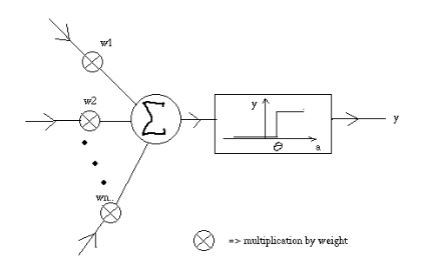
\includegraphics[width=8cm]{images/mccullochneuron.JPG}
\caption{McCulloch Neuron}
\label{fig: Machine neuron}
\end{figure}

\begin{figure}[htp]
\centering
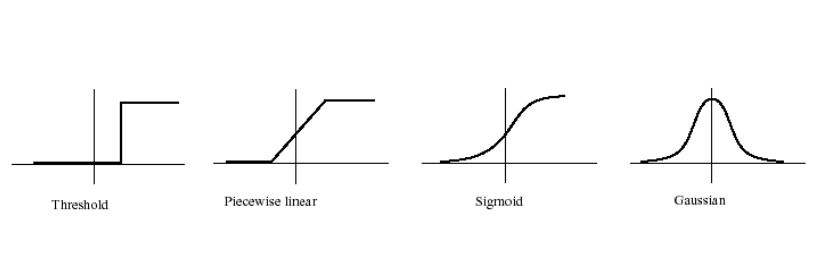
\includegraphics[width=15cm, height=6cm]{images/activationfunctions.JPG}
\caption{Activation Functions}
\label{fig: Act func}
\end{figure}

\textbf{Relation of Hebbian Learning and Artificial Neural Networks:} \\
Hebbian Learning or Associative Learning: Useful neural connections get strengthened over time, and not so useful ones die out. When neurons fire together, they wire together. \\
ANN Works similarly, where the system learns the irght weights (signifying the importance of a feature from the training data through \textbf{back propagation}. With training the weights of useful features in the network get strengthened (increase in value), and those of not so useful ones get weakened (decrease in value). This learning process is similar to Hebbian learning in the sense that the weights are determined though iterations of learning and reinforcement/punishment. \\

\textbf{Examples of Artificial Neural Network:} 
\begin{figure}[h]
\centering
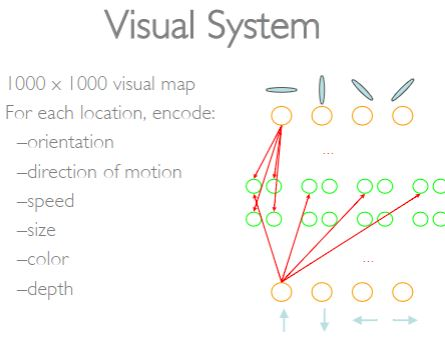
\includegraphics[width=6cm]{images/visualsys.JPG}
\caption{Visual System}
\label{fig: vissys}
\end{figure}

\begin{figure}[h]
\centering
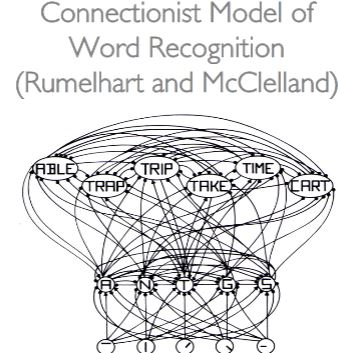
\includegraphics[width=6cm]{images/connectionist.JPG}
\caption{Connectionist Model of Word Recognition}
\label{fig: connectionist}
\end{figure}

\begin{figure}[htb]
\centering
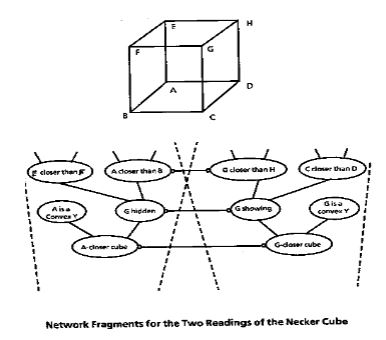
\includegraphics[width=5cm]{images/necker.JPG}
\caption{Necker Cube}
\label{fig: Necker}
\end{figure}


\subsection{Perceptrons}
The simplest kind of "feed forward" neural network. (Originally introduced by Frank Rosenblatt (1985).\\
\textbf{Feed Forward}, refers to the direction in which information/data flows when the neural network is making a prediction, i.e. input layer $\rightarrow$ hidden layer $\rightarrow$ output layer. Features come in from the input layer, the information flows through the network and the system generates some output (some predition/classification result) at the end\\
\textbf{Back Propogation}, refers to the direction in which error/ update flows when the system is learning. During the training stage, we have the data of both the input and desirable output. For a given input, the system compares its prediction with the desirable output, and use  the difference/prediction error to update the network (hebbian learning). This error is therefore fed backward through the system, so the weights in the networks can be adjusted accordingly. The goal is that with these adjustments, the network will learn from its mistakes and give better and better predictions. \\
\textbf{Multilayer Feed Forward Network:} Consists of \textbf{hidden layers} which are these weights that determine the output layer. If the output is not desirable, back propagation is used to adjust the weights in the hidden layer. \\

\begin{figure}[htp]
\centering
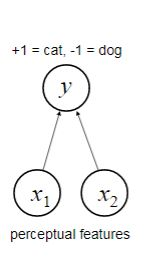
\includegraphics{images/perceptron.JPG}
\caption{Perceptron Simple Feed Forward}
\label{fig: Perceptron}
\end{figure}


\begin{figure}[htp]
\centering
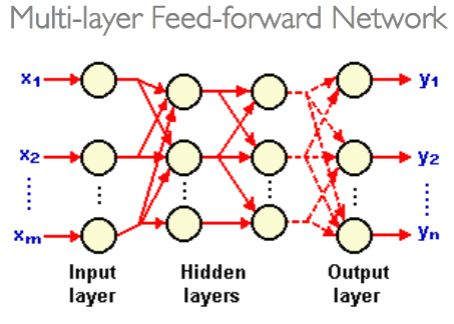
\includegraphics[width=5cm]{images/multilayerfeedforward.JPG}
\caption{Multi-Layer Feed Forward}
\label{fig: MLFF}
\end{figure}

\begin{figure}[htp]
\centering
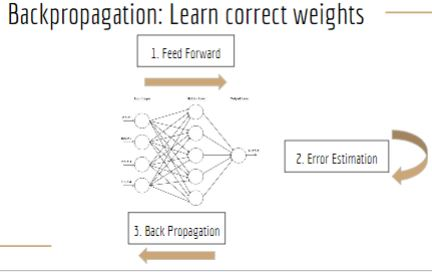
\includegraphics[width=10cm]{images/backprop.JPG}
\caption{Backpropagation}
\label{fig: back prop}
\end{figure}

\newpage
\section{Lecture 13: Guest Lecture Anand Kulkarni on AI}

\textbf{Takeaways:}
\begin{itemize}
    \item What is AI?
        \subitem Study and Engineering of making machines intelligent. Intelligence is broad, but we'll compare it to behaving like a human
        \subitem A.I. is a moving target, we used to think of Chess A.I. as significant, but now we have Google maps and translate and we don't even think of it as A.I. 
    \item Neural Network
        \subitem Model the machine like a brain
        \subitem Brains have neurons, so we make machine neurons, known as Perceptrons
        \subitem Perceptrons are Linear binary classifiers. Linear because we multiply our inputs by weights and then sum them together linearly. (no squared or cubed) And then binary because when we output either a 1 or 0. 
        \subitem Take inputs, multiply by weights and sum them, run through unit step function(activation function). Tells us what the neuron does in response to our input 
    \item Feature sets
        \subitem Build neurons using feature sets (weights). 
        \subitem Features relate to the function we want our A.I. to perform (Ex: We want computer vision, so we need to detect colors, orientation, motion, shape, depth, etc. These are our features)
    \item Deep Learning
        \subitem Multiple-layers in our neural network (i.e. layer is made of multiple perceptrons. Having multiple layers of these perceptrons simulates how neurons send signals to more neurons)
        \subitem Feed Forward Neural Network, goes in one direction. 
    \item AI risks
        \subitem Concerned about bias in our data. 
        \subitem Like a naive human, our A.I. is also naive to something, so we train it with a data sets and back propagation. 
        \subitem However, we want to make sure our data is not biased as well. 
\end{itemize}

\newpage
\section{Lecture 14: "Playing with Perceptrons" (Neha Mittal)}
\textbf{Arthur Samuel} - Father of Machine Learning \\
\indent Created A.I. checker player that beat the checkers champion \\

\noindent \textbf{A.I. Today:} Google search, Facebook Graphs, Amazon Recommendations \\

\subsection{B.F. Skinner's Radical Behaviorism Theory}
Look back to Lecture 9 for definition. \\
\textbf{Machine Learning:} gives computer systems the ability to "learn" with data and not much programming. \\
\textbf{Computer Vision:} Making computers see as humans do. Involves acquiring, processing, analyzing and understanding images and extraction of high dimensional data. \\
\begin{figure}[htp]
\centering
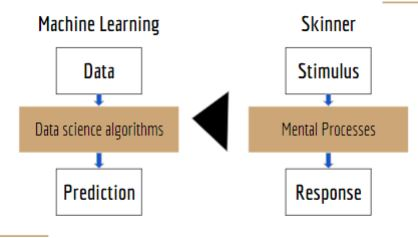
\includegraphics[width=9cm]{images/machinelearning.JPG}
\caption{BF Skinner in relation to Machine Learning}
\label{fig: ML and Skinner}
\end{figure}

\noindent \textbf{Concepts of Machine Learning:} 
\begin{enumerate}
    \item Input(x) and Output(f(x) or y
    \item Classification of Output
    \item Learning aka Training
    \item Training vs Testing Phase
\end{enumerate}

\noindent \textbf{Problems with traditional ML Models:}
\begin{enumerate}
    \item Domain Knowledge
    \item Infinite variations of inputs
\end{enumerate}

\noindent \textbf{Main Concepts of Lecture:}
\begin{itemize}
    \item Featurization
        \subitem These are the weights in our ML neural net. Weighted differently based on importance
    \item Perceptrons: Feed Forward Calculations
        \subitem In the image below, multiply weight by input and sum the weights. 
        \subitem Then we get an activation function which will determine the output. 
    \item Success of deep learning in computer vision: loads of image data made open source \textbf{architecture by hand} instead of feature design by hand
        \subitem \textbf{Feature by Hand:} Focus is ensuring the usefuelness/quality of the features. 
        \subitem \textbf{Architecture by Hand:} Just want to make sure your features are expressive/ contain useful information. Main focus is designing the best architecture that will allow the useful bits in your feature to shine and help you generate the best output.
        \subitem \textbf{Example: predict students grades} \\
        \textbf{Feature by hand:} solve focusing with \textbf{high quality features} that are predictive of students performance, e.g. midterm grades. \\
        \textbf{Architecture by hand:} solve with \textbf{many features} about a student, e.g. midterm scores, breakfast, commute, shoes. 
        \subitem Point is that hopefully the Neural Network will figure out which features are most predictive of the scores drawing from huge data sets. 
        \subitem Example from class: Geoff Hinton and Image Net, Paul Li described as cute
    \item Difference between perceptron and deep learning
        \subitem Perceptron is like the single-layer perceptron earlier in the study guide. It has one hidden layer, which is shallow. 
        \subitem Deep learning is like the Multi-layer feed forward network, where it has multiple hidden layers that take inputs from the previous layer. Deep because of its depth in layers. Look at backpropagation as well. 
\end{itemize}
\begin{figure}[htp]
\centering
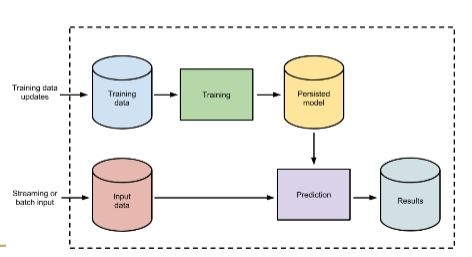
\includegraphics[width=15cm]{images/MLconcept.JPG}
\caption{ML training}
\label{fig: ML}
\end{figure}

\begin{figure}[htp]
\centering
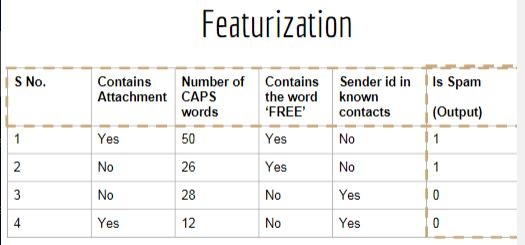
\includegraphics[width=15cm]{images/featurization.JPG}
\caption{Featurization}
\label{fig: featurization}
\end{figure}

\begin{figure}[htp]
\centering
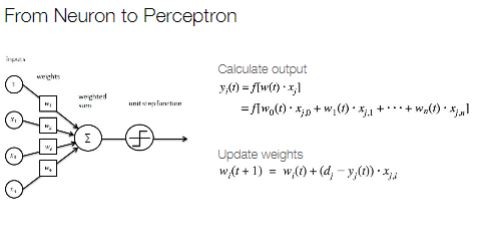
\includegraphics[width=15cm]{images/feedforwardcalc.JPG}
\caption{Perceptron Calculation}
\label{fig: calc}
\end{figure}

\begin{figure}[htp]
\centering
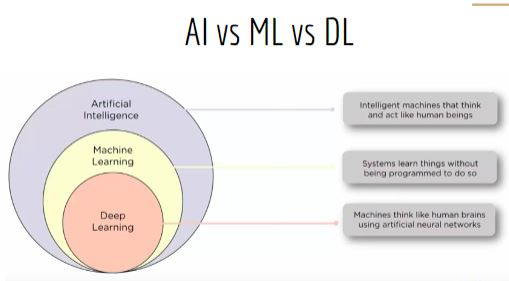
\includegraphics[width=15cm]{images/AIMLDL.JPG}
\caption{AI vs ML vs DL}
\label{fig: aimldl}
\end{figure}

\begin{figure}[htp]
\centering
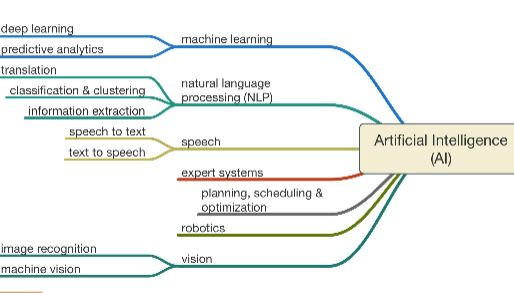
\includegraphics[width=15cm]{images/AI.JPG}
\caption{AI}
\label{fig: ai}
\end{figure}

\section{Lecture 15: The Philosophical Approach: Consciousness}

\subsection{Lucid Dreaming defined by Paul Tholey}
7 factors to fulfill \\ 
\textbf{Awareness of...}
\begin{enumerate}
    \item the dream state (orientation)
    \item the capacity to make decisions
    \item memory functions
    \item self
    \item the dream environment
    \item the meaning of the dream
    \item concentration and focus (the subjective clarity of that state) 
\end{enumerate}

\section{The Mind-Body Problem}
\begin{itemize}
    \item The \textbf{brain} is material and physical and can be studied objectively
    \item The \textbf{mind} consists of subjective phenomena such as thoughts, feelings, and beliefs
    \item What is the relationship between the two?
\end{itemize}

\noindent Brings forth two ideas: 
\begin{itemize}
    \item \textbf{Monism:}            
    \subitem Aristotle (384-322 B.C.) advocated a physical form of monism. He believed the mind and body were both physical. 
    \item \textbf{Dualism:}
        \subitem Plato (427 - 347 B.C.) was a dualist
        \subitem Dualists, who see mind as separate from body, claim that consciousness is a property of spiritual minds and is not open to scientific explanation. 
\end{itemize}

\section{Consciousness}
\textbf{Definition:} may be defined as the subjective quality of mental states \\

Even the dictionary does not have a clear definition of consciousness. (\textbf{may be)} \\ 

\noindent \textbf{Etymology}
\begin{itemize}
    \item The origin of the modern concept of consciousness is often attributed to John Locke's Essay Concerning Human Understanding, published in 1690. Locke defined consciousness as "the perception of what passes in a man's own mind". 
    \item Samuel Johnson's definition of "consciousness": "the opinion or internal feeling that we ourselves have from what we do."
    \item English word "conscious" derived from Latin conscius (con - "together" and scio "to know"), meant "knowing with" in Latin or "having joinnt or common knowledge with another". 
\end{itemize}

\noindent Conscious mind is only 10\% while subconscious mind is 90\%. \\
No problem can be solved from the same level of consciousness that created it - Albert Einstein \\ 

\nondent \textbf{Searle definition:} \\
The 'mystery' of consciousness today is in roughly the same shape that the mystery of life was before the development of molecular biology... It seems mysterious because we do not know how the system of neurophysiology/ consciousness works, and an adequate knowledge of how it works would remove the mystery. \\

Basically, if we figured out what consciousness is, we would know what consciousness is. Some circular loop. \\

So what do we know about consciousness? \\ 
\begin{itemize}
    \item We know the visual pathways: Dorsal and Ventral
    \item We know how this information travels throughout the brain
    \item We know the physical biology of the brain and how we learn, how we transfer memory, etc. 
    \item We know that the brain has synchronized background neuronal activity at 40Hz due to EEG on subjects during REM and unconscious states. 
    \item The brain is sort of always on all the time, this area is still gray (unknown) in its function of our physiology. 
\end{itemize}

\noindent \textbf{Emergent Properties:} the mind may be an emergent property of the brain. \\

Just as water emerges from the interaction of H2O molecules but cannot be explained entirely by their individual properties, so is the brain. \\

\subsection{CRUM and Consciousness}
We use this idea of the CRUM (computational representational understanding of the mind) model to tell us how the mind works by using computational representations to understand the mind. \\ 

\noindent \textbf{Neurocomputational Theory of Consciousness} \\
Consciousness is caused by 3 mechanisms: 
\begin{enumerate}
    \item \textbf{Biological/ Neurological}
        \subitem Since blows to the body other than the head are unlikely to cause loss of consciousness, evidence from coma, concussions, and fainting suggest that consciousness must be neurological. \subitem Consciousness stops when the cellular processes of energy metabolism cease. 
    \item \textbf{Electrical}
        \subitem Epilepsy is a group of disorders that involved alteration or loss of consciousness
        \subitem Epileptic seizures are accompanied by \textbf{abnormal electrical activity} in the brain
        \subitem We lose consciousness every day when we all asleep, which is marked by electrical changes
    \item \textbf{Chemical}
        \subitem Adenosine promotes sleep and decrease wakefulness
        \subitem Caffeine, an antagonist for adenosine receptors, promotes wakefulness
        \subitem Other neurotransmitters involved: dopamine, histamine, noradrenaline, serotonin, and GABA
\end{enumerate}

\textbf{Ideas of consciousness:} \\
\begin{itemize}
    \item Crick and Koch 1995: Consciousness may be the product of specialized consciousness neurons
    \item Popper and Eccles 1981: Consciousness is the emergent property of neuronal activity
    \item Other theories postulate the existence of corticothalamic circuit in which information is passed recurrently between the cortex and thalamus
\end{itemize}

\subsection{Neurologic disorders related to consciousness} 
\begin{itemize}
    \item Posoopagnosia and other agnosias: inability to process sensory information
    \item Blindsight: Can't physically see, but motion detectors of eyesight still active
    \item Visual Neglect: damage to one side of the hemisphere which causes neglect of the contralateral side
\end{itemize}

\section{Lecture 16: Puzzle of the Bandwidth of Perceptual Experience by Greyson Abid}
\textbf{Rich perceptual experience:} we usually have a sense that we enjoy a richly detailed visual experiences, high-fidelity experiences that extend to objects in your periphery \\ 
Ex: Autobiographical example: Coit Tower in San Francisco \\

\noindent Is it possible that we are mistaken about what we see, that we aren't actually seeing all that is there? \\

\subsection{Puzzles}

\begin{enumerate}
    \item \textbf{Blind spot:} region of visual field corresponding to the optic nerve and blood cells that leave the retina. (no photoreceptors present here) 
    \begin{itemize}
        \item You can become aware of this, but there isn't a black spot in your vision. 
        \item Possibility 1: blind spot "filled-in" by the brain (Ramachandran, 1992)
        \item Possibility 2: blind spot ignored by the brain (Dennett, 1991)
        \item No reason that the brain must "fill-in" the spot, but evidence suggest it does do some neural filling-in
        \item \textbf{P1:} Ehinger et al. (2017) two patches: one continuous, one not. Non continuous one was filled in by blind spot. More likely to judge as filled in even if the other patch was continuous. \\
        Subjects preferred 'seeing' within their blind spot over seeing outside of it
        \item \textbf{Naive interpretation:} the patch containing an inset within the blind spot is consciously perceived as being more continuous than the patch completely outside of the blind spot
            \subitem Under this interpretation, subjects judged that the patch with an inset contained in the blind spot was more continuous because it appeared more continuous. 
        \item \textbf{Unconscious bias interpretation:} the preference for the blind spot reflects an unconscious bias on the part of the subjects
            \subitem Naive interpretation seems right, but not directly supported by the experiment results
    \end{itemize}
    
    \item \textbf{Visual crowding:} when an object in the periphery is surrounded by distractors (i.e., "flankers") 
        \begin{itemize}
            \item Objects identifiable if displayed in isolation but are not easily identified when placed in a crowded display
            \item \textbf{P2:} Odegaard et al. performed a two-alternative forced choice task in which subjects reported the orientation of a briefly presented patch and then gave a scaled confidence rating of their judgment 
            \subitem "single" condition, the patch is presented in isolation. 
            \subitem "crowded" condition, it is crowded by two flankers
            \item subjects performed worse in crowded condition
            \item Participants overconfident in crowded, but not in the single condition 
            \item High confidence for incorrect trials, participants don't know they are wrong and have more confidence in their perceptions than is warranted
            \item Subjects explicitly provide confidence ratings corresponding to their judgments, this result, along with the next, conflicts with an unconscious bias interpretation
            \item \textbf{Naive interpretation:} high confidence ratings correspond to high apparent visibility 
                \subitem Across incorrect trials in the corwded condition, subjects "see" the incorrect orientation of the crowded patch
            \item Alternative interpretation: experiment concerns inflated \textbf{confidence} ratings, which may not reflect what subjects visually experience
            \item \textbf{Skeptical interpretation:} the subjects' confidence ratings do not tell us anything about subjects' visual experiences
                \subitem Cannot be dismissed offhand because confidence and visibility can diverge
        \end{itemize}
    
    \item \textbf{Change blindness:} subjects fail to notice significant changes that unfold directly in front of them
        \begin{itemize}
            \item partially the result of a failure to attend since changes are noticed more easily if attention is drawn to the location of the change. Nevertheless, the phenomenon may also reflect a failure of comparison
            \item \textbf{Overflow interpretation:} change blindness reflects a lack of cognitive access but does not reflect a limit on perceptual experience. Under this view the phrase 'change blindness' is a misnomer (it's there, but we just don't consciously acknowledge it) 
            \item \textbf{P3:} Grating detection and discrimination tasks, measured detection biases and visibility ratings as a function of attentional cuing
            \item Discrimination tasks, subjects gave higher visibility ratings in conditions of reduced attention (sensitivity was lower in conditions of reduced attention for all contrasts) 
            \item \textbf{Naive interpretation:} take subjects' visibility ratings at face value
                \subitem Accept that apparent visibility is higher in conditions of reduced attention, even though discrimination sensitivity is lower in these conditions \subitem Change blindness is explained in a special instance of this phenomenon: visibility is high in unattended parts of a scene, but detection sensitivity is low
            \item \textbf{Skeptical interpretation (redux):} subjects' visibility ratings are not a guide to apparent visibility in conditions of reduced attention
        \end{itemize}
\end{enumerate}

\subsection{Methodological considerations}
\textbf{Methodological consideration:} if a range of subjects systematically report that they experience P, then we have \textit{prima facie} reason to believe that they experience P. Thus we need a motivation for skeptical interpretation. 
\begin{enumerate}
    \item \textbf{Motivation for Skepticism 1:} Maybe these results reflect a "hypertrophy of confidence" due to lack of feedback \\
    \textbf{Reply:} This does not seem to be the case. These effects were rigid: they were not altered by changing the task payoff or by giving increased feedback (P3), and do not appear to be the result of response bias (P1). 
    \item \textbf{Motivation for Skepticism 2:} there is a more general trend that subjects are systematically mistaken about their own experiences. For instance, "firmly established" that we have poor color vision in the periphery \\ 
    \textbf{Reply:} We do not have poor color vision in the periphery! Results suggesting otherwise do not take into account cortical magnification. 
    \item \textbf{Motivation for Skepticism 3:} if naive introspection were a reliable guide to visual experience, then one would expect widespread agreement about phenomenology. Nevertheless, we find widespread disagreement. Thus we ought to be skeptical. \\
    \textbf{Reply:} Why think there is a widespread disagreement about naive introspection? of course, widespread disagreement is found among philosophers and psychologists, but this is still likely an artifact of response bias, which can be controlled for experimentally
\end{enumerate}

\noindent Visual experience doesn't always accurately represent the world (constant illusion)? Examples are ubiquitous in our visual lives. \\ 

\textbf{bold claim:} visual experience often informs us about the world, but it is not the sort of things that can be accurate or inaccurate; visual experience is a matter of construction (like building a house using availble materials rather than painting a portrait).  

\section{Lecture 17: Explaining Consciousness by Geoffrey Lee}
Philosophy of Mind: \\
\begin{itemize}
    \item \textbf{Empirical Psychology:} the scientific study of the mind/ brain
    \item \textbf{Folk Psychology:} our everyday ways of talking and thinking about the mind
\end{itemize}
The relationship between these two in my opinion is that we sort of need both to think about the mind and the brain. We need to understand it from both a scientific and social aspect. \\ 

\noindent \textbf{Nagel's Definition:} a mental state is conscious just if there is "something it's like" to have that mental state. \\ 
Other kinds of consciousness: self consciousness, access consciousness \\ 

A couple questions on the science of consciousness: How can we tell if something is conscious? (such as an octopus, animal, robot, etc). Is there a systematic connection between physical /structural features of the brain and the features of conscious experience? \\

\begin{itemize}
    \item \textbf{Reductionism:} consciousness is a special kind of complex processing in the brain (must be broken down into parts that we must analyze to understand)
    \item \textbf{Supervenience:} no difference in consciousness without differences in the brain (consciousness is fully determined by the brain)
    \item \textbf{Psychophysical Laws:} Laws systematically linking conscious states with states of the brain
    \item \textbf{Neural Correlates of Consciousness (NCC):} What are the neural bases in humans of particular kinds of conscious experience?
\end{itemize}

\noindent Bincoular Rivalry (Tong et al. 1998): This experiment tests the red/green 3d glasses and you can consciously switch which image you are looking at, the face or the house. They also show the activation of two separate areas, the Fusiform Face Area (FFA) and Parahippocampal Place Area (PPA). Both are stimulated yes we can shift our percept. 

\subsection{Obstacles to explaining consciousness}
\begin{itemize}
    \item \textbf{Easy Problem of consciousness:} the problem of explaining how functions that are associated with consciousness - (for example, the ability we have to discriminate and report information about our environment) - are implemented in the brain
    \item \textbf{The Hard Problem:}  suppose we know that brain state B is necessary and sufficient for having experience E. Why does B go with E rather than some other type of experience? Why is B associated with experiences at all? 
    \item \textbf{Methodological Puzzle:} the science of consciousness requires correlating experiences with brain states. But how do we tell what experiences someone is having during an experiment? (no direct tests, rely on indirect tests like verbal reports) \\
    \textbf{The puzzle:} how do we distinguish the neural mechanisms relevant to our access to consciousness from those directly relevant to consciousness itself? (distinguish experiences that are relevant to consciousness vs access to consciousness) 
\end{itemize}

\subsection{Rich vs Sparse View}
\begin{itemize}
    \item \textbf{Rich view:} a conscious visual experience can contain a richer array of information than is accessed/ immediately accessible 
    \item \textbf{Sparse View:} the only information that is conscious, is information that is accessed /accessible
    \item Sperling's experiment: did this in Konlin's section. Flash array of letters. Auditory tone and line to remember. Repeat cued line
\end{itemize}

\subsection{Consciousness vs the Consciousness role}
\begin{itemize}
    \item \textbf{Heterophenomenology:} the project of determining what people believe (or say) about their experiences
    \item \textbf{The Consciousness role:} a systematized description of the role that consciousness plays in our mental lives, based on what we believe (or say) about it. 
    \item \textbf{A tractable project:} spell out the consciousness role, and then figure out what natural phenomenon best satisfies it
\end{itemize}

Questions that could trouble the consciousness role projects: 
\begin{itemize}
    \item \textbf{Multiple best candidates:} what if there are many equally good candidates for what plays the consciousness role in humans? 
    \item \textbf{Different realizers in other beings:} what if an alien or AI has a state that plays something like the role that consciousness plays in us, but it's not a state we have (so it's not consciousness?)
    \item \textbf{Deflationary Pluralism:} even if a being lacks consciousness, it can have a state that plays a similar role, and is just as significant as consciousness. 
    \item Forms of significance: Natural, Epistemic, Moral/ Practical
\end{itemize}

\section{Lecture 18: Learning is Moving in New Ways: \\ Building Educational Theory Through Design-Based Research on Embodied Mathematics Cognition and Instruction \\ by Dor Abrahamson}

\subsection{Investigative Approach: Design-based Research: }
Conjecture-driven, iterative, empirical studies, wherein, theory and design, co-inscribe. \\
Creating designs for young people, young minds, for people to learn. \\

\textbf{How embodied design started:}\\
\begin{itemize}
    \item 1837: Beginning of Kindergarden 
    \item People who sort of inspired this idea throughout the years from 1782 to 1928: Friedrich Frobel, Maria Montessori, Hans Freudentahl, Caleb Gattegno, Zoltan Dienes, Seymour Papert
    \item Example: Gave kids toys and gifts to learn in a motor way.
\end{itemize}

\begin{itemize}
    \item \textbf{Embodied Design:} constructing means for constructing meaning. Make the concepts exist in the childrens minds. 
    \item CRUM giving them concepts so they may able to draw meaning, make into propositions, images, analogies etc
    \item Experience first, analyze later: building mathematical concepts form perception, action, aesthetics, and common sense. 
\end{itemize}

\noindent\textbf{Embodied Mathematical Reasoning: } \\
Terrence Tao: math professor at 24. \\
He imagined things using imagery and motion to help him solve problems such as: Egg frying in a pan of oil, Jet ski riding  a wave in the ocean, Rolling on the floor

\subsection{Enactivism}
\textbf{Enactivism (Varela, Thompson, and Rosch):} "in a nutshell the enactive approach consists of two points:
\begin{enumerate}
    \item Perception consists in perceptually guided action; and
    \item Cognitive structures emerge from the recurrent sensorimotor patterns that enable action to be perceptually guided."
    \item example: proportion: wii sensors where the left side had a proportion of 1 and the right 2. So to make the screen green, right side had to be 2x the left. \\
\end{enumerate}

Learned techniques to help learn: 
\begin{itemize}
    \item \textbf{attentional anchors} 
        \subitem use of Patrick McCaw syllables to produce a (3) slap and (2) snap pattern
        \subitem used DUET (dual eye tracking) and eye tracking studies with the 1:2 ratio experiment (both parallel and orthogonal) and found that as kids found the hook and shift, they used attentional anchors to keep that proportion. (watching the diagnol, making a rectangle) 
    \item \textbf{hooks and shifts} 
        \subitem A hook is a subjective and contextual affordance of a mathematical artifact that students recognize as they become cognizant of the artifact’s availability in the course of solving a problem and communicating their solution. (wii ex: must hold hands at 1:2 ratio to turn screen green)
        \subitem A shift is the students’ consequent, unpremeditated and undemonstrated yet more mathematically sophisticated analysis of the problem situation that emerges through using the artifact (wii ex: must keep the shift at a 1:2 ratio to keep screen green) 
\end{itemize}

\section{Lecture 19: Persepectives of Anthropology by Tracy Brannstorm}

\subsection{Sub-fields of Anthropology}
Main one's to focus on, biologial and cultural 
\begin{enumerate}
    \item \textbf{Cognitive Archaeology:} Studying the human mind from past societies through their material remains
        \subitem groups of people living together tend to develop a shared view of the world and similar cognitive maps which in turn influence their material culture
    \item \textbf{Biological:} Links social behavior to biology
        \subitem Evolution of human brain and consciousness
        \subitem Primate behavior \\
        \textbf{Evolutionary Psychology:}
            \begin{itemize}
                \item Evolutionary approach to understanding human behavior and mind 
                \item How and why did human intelligence and consciousness evolve? 
                \item Evolution: the process of change in a species that occurs over many generations, throught natural selection
                \item Disease-avoidance mechanism
            \end{itemize}
        \subitem Very hard to prove evolutionary mechanisms for ethology
        \subitem Useful case study is the domestication of silver foxes in Russia. It was illegal to do evolutionary studies in Russia, but this person had the foxes for their pelts. So he ended up taking the most docile foxes to breed while turning the rest into fox pelts. He ended up creating a breed of silver foxes that can be domesticated. 
    \item \textbf{Linguistic Anthropology}
        \begin{itemize}
            \item How do language and culture interact? 
            \item Sapir-Whorf Hypothesis: "Grand generalizations of Western World, such as time, velocity, and amtter, are not essential to the construction of a consistent picture of the universe" 
            \item Daniel Everett et al. (2008): 
                \subitem Piraha have no words for expressing exact quantities or colors
                \subitem Suggests that language is a cultural invention rather than a linguistic universal
        \end{itemize}
    \item \textbf{Cultural Anthropology:} Looking for \textbf{shared realities}: knowledge, behavior, interactions, experience, language, and \textbf{meaning}
        \begin{itemize}
            \item \textbf{Context}: how different social and cultural contexts shape a person in various ways - cognition, etc. 
            \item Individuals respond to and interact with cultural materials and contexts, but culture is also responsive to, and created by, the ways that individuals enact it. The direction of influence is two-way - "looping" 
            \item Looking for the specific rather than general
        \end{itemize}
\end{enumerate}

\subsection{Tracy Brannstorms Work as a Cultural Anthropologist}
\begin{itemize}
    \item Collect \textbf{qualitative} data (quantitative as well) 
    \item Any information that can be captured that is not numerical in nature (e.g. perceiving relationships) 
    \item Fieldwork Methodology: interviews, [participant] observation, surveys
        \begin{itemize}
            \item researcher studies a society from the point of view of that society, meaning they derive from their experiences living in the society 
            \item researchers using their bodies and minds as primary tools
            \item "human experience cannot be measured in a lab. It's too private, fluid, specific, idiosyncratic, difficult to capture and predict (wild). 
        \end{itemize}
\end{itemize}

\textbf{Why does cultural anthro matter?} 
\begin{itemize}
    \item 2010 a study on studies found that 96\% used Western subjects
    \item \textbf{WEIRD} subjects (Western, Educated, Industrialized, Rich, and Democratic): 
        \subitem from countries that represent about 12\% of the world's population
        \subitem differ from other populations in decision making, reasoning, visual perception, etc. 
    \item essentially it's dangerous to generalize subjects in Western culture to the rest of the world, because it's not representative. (selection bias lel) 
\end{itemize}

\subsection{Plants and Cognition/consciousness}
\begin{itemize}
    \item \textbf{Sedge} plant from Machiguenga culture
        \subitem has many uses such as monkey hunting, childbirth, warfare and medicine
    \item \textbf{Ayahuasca} made from boiling 2 types of plants
        \subitem Alters consciousness (not defect, but valued) 
        \subitem Used in diagnosis and treatment
\end{itemize}

\noindent \textbf{Plants}
\begin{enumerate}
    \item Banisteriopsis, Caapi (or ayahuasca)
        \subitem \textbf{Active components:} Harmine (telepathine), Harmaline, , Tetrahydroharmine
    \item Psychotria Viridis \textit{Chacruna}
        \subitem \textbf{Active components:} Dimethyltryptamine (DMT) 
        \subitem close analogue of serotonin
        \subitem exists naturally in the mammalian brain, inn 100+ plants and animal species (but why? Dunno) 
\end{enumerate}

\textbf{Ritualized context}
\begin{itemize}
    \item Sessions at night, lasting many hours
    \item with few people or large groups
    \item drink for multiple reasons
    \item Practitioners and patients both consume it (healing crisis) 
    \item use tobacco and other plants as well
    \item Music can be used in rituals such as these, and they help bring on, take away, or change content of visions
\end{itemize}

The reasons for these rituals is really unknown because it's really got nothing to do with reproduction, just as art, music, literature, humor, politics etc. \\

\subsection{Scientific Research of Ayahuasca}
\begin{itemize}
    \item Sat Pau University, Barcelona
    \item How do active substances in vine (harmine and tetrahydroharmine) affect neurons directly
    \item Alkaloids stimulated creation of neurons (neurogenesis)
    \item Reduced neurogenesis has been linked to higher stress levels and depression
    \item MRI images of 22 regular + 22 controls
    \item Shrinking in brain region, \textbf{posterior cingulate cortex} (PCC) 
    \item PCC is part of brain's \textbf{default mode network} (DMN), regions involved in selfhood processing
    \item Hyperactivity in this region associated with pyschopathology like depression
    \item Recent use of EEG to measure brainwaves of subject under ayahuasca effects
    \item Found reduction in alpha waves in PCC, major part of DMN
    \item Past research correlates alpha activity to conceptions of self. 
\end{itemize}

\noindent \textbf{Pyschedelic Renaissance}
\begin{itemize}
    \item Began in 90s
    \item Study of psychedelics to learn about
        \subitem biological substrates of mental illness
        \subitem Neurotransmitter systems
        \subitem Neural correlates of consciousness
    \item US, Switzerland, Germany, Spain, Russia, etc. 
    ]item PBS called this research 'forefront of a revolution in neuroscience and medicine"
\end{itemize}

\section{Lecture 20: Cognitive Science and Digital Technologies by Todd Davies}

Todd Davies spoke about broadcasting messages and how digital technology has affected the social sciences. \\ 

\begin{itemize}
    \item "The medium is the message" - Marshall McLuhan
    \item The \textbf{medium} in which you send information has an impact on how the message is received
        \subitem The scale of human activity
    \item McLuhan had this idea of a global village, which is the metaphoric shrinking of the world through electronic media 
    \item In short: digital technology makes us more dependent on mental shortcuts causing fatigue, rush and overload, and overall making us less happy and more depressed
    \item Money improves happiness of poor but not for non-poor - Richar Easterlin (1974) 
\end{itemize}

\noindent \textbf{Psychological Mechanisms:}
\begin{itemize}
    \item \textbf{Loss aversion:} people's tendency to prefer avoiding losses to acquiring equivalent gains
    \item \textbf{Myopic decision making:} tendency in decision makers to focus on information immediately related to their judgment and to ignore other, less prominent, pieces of information 
    \item \textbf{Hedonic treadmill:} - adaptation to new wealth, tendency of humans to quickly return to a relatively stable level of happiness despite major positive or negative events or life changes
\end{itemize}

\noindent Deep Dive: Online Diffusion \\
Two case studies: one of Twitter messages and one of Petition messages, to measure their virality. 

\begin{itemize}
    \item Structural virality: either a broadcast or viral structure. (message comes from one node and sent to many or message spread across many nodes in a tree like structure) 
    \item Intrinsic virality: How much meaning is in the message that causes it to become viral. 
    \item Structural virality does not imply intrinsic virality/infectiousness
\end{itemize}

\noindent \textbf{Exceed ratios:} inverse indicators of structural virality 
\begin{itemize}
    \item \textbf{Total exceed ratio:} 
    \begin{equation}
        E_{Tot} = \frac{\Sigma_{i \in L}(S(i) - max[S(i-1), S(i+1)])}{\Sigma_{i = 1}^T S(i)}
    \end{equation}
        \subitem for a given petition over T time periods, in which S(i) signatures are obtained in period i, and L is the set of all peak periods within T (measure the peaks within the graph and divide them) 
        \subitem Shown that unsuccessful petitions had higher total exceed ratios for daily and hourly by almost 50\%
    \item \textbf{Global-peak-only-exceed ratio} $E_{GPO}$ = adjacent-periods signature difference for just the global peak period divided by total signatures (an indicator of the largest broadcast event) (measure the largest event) 
        \subitem Same results when measuring daily global peak only exceed ratios, where the unsuccessful petitions had over 50\% ratios. 
\end{itemize}

\noindent \textbf{First day/ second dat (FDSD) ratio:} an indicator of intrinsic virality \\
Assumptions:
\begin{itemize}
    \item Most petitions are launched by some kind of broadcast event on the first day 
    \item Therefore, petitions that achieve more signatures on the second day than on the first day will be, on average, higher in intrinsic appeal than those with higher FDSD ratios. 
    \item More petition signatures on the second day usually indicate a more successful petition because it signifies the intrinsic virality is higher (message has more meaning) and that is why it gains more traction after the first broadcast event. 
\end{itemize}


\end{document}